\chapter{Analysis and Design}
\label{chap:analysis-design}

Leveraging the notions coming from \Cref{chap:background}, this chapter inspects the current state of aggregate computing, identifying some of the missing features of the current model as proposed by field calculus (\Cref{sec:current-state}).
%
Subsequently, \Cref{sec:proposed-model} describes a prototype of a \textit{reactive model} for aggregate computing, introducing the objectives and giving a preliminary analysis of how the proposed model is expected to fulfill them.
%
Finally, \Cref{sec:specification} presents the major design choices that were taken prior to implementation.

\section{Analysis of the current state}
\label{sec:current-state}

In order to have a comprehensive view on the subject, this section provides a brief analysis of the current state of aggregate computing, first by describing the \textit{proactive model} and identifying its limitations, then by introducing \textit{ScaFi}

\subsection{Proactive model}

At the current stage, field calculus and aggregate computing are based on a model where each device of the network \textit{repeatedly} executes its computation in rounds of \textit{sense-eval-broadcast}.
%
In particular, referring to the model discussed in \cite{10.1145/3177774}, each sense-eval-broadcast round of a device is alternated with some \textit{sleeping time} during which it collects information from neighboring devices.
%
This way of managing computation can be thought of as a \textit{proactive model}, since its the device that decides when computation should occur based on its internal scheduler.

The proactive model has some shortcomings.
%
On the one hand, there is no way to granularly control the \textit{timing} and the \textit{dynamics} of computation rounds using the main operators of field calculus alone.
%
In fact, there is often the need to perform computation upon the occurrence of particular events, for example when a sensor changes its value, or when a message is received from a neighbor.

On the other hand, since computations are carried out regardless of the existence of significant changes in the environment or in the knowledge of the neighborhood.
%
In turn, this implies that the \textit{broadcast} step is also carried out even if there is no change in the generated export, resulting in \textit{wasteful message exchange}.

The shortcomings of the proactive model call for a more \textit{reactive approach}, where taking actions only upon significant changes is a pivotal concern and should be taken into account as first class in the supporting model.
%
A prototype for this is presented in \Cref{sec:proposed-model}.

\subsection{ScaFi}

This section presents a brief introduction to \textbf{ScaFi}, a Scala-based library and framework for aggregate programming \cite{scafi-docs}.
%
In particular, the \textit{API} and the \textit{core} of ScaFi will be analyzed in order to facilitate both the design and implementation stages, since they can be used as references to guide the whole process.

ScaFi's API is heavily inspired by the field calculus' language and consists of a trait defining the main constructs that can be used to describe aggregate computations:
%
\begin{lstlisting}[frame=single, language=scala]
trait Constructs {
  def nbr[A](expr: => A): A
  def rep[A](init: =>A)(fun: (A) => A): A
  def foldhood[A](init: => A)(aggr: (A, A) => A)(expr: => A): A
  def aggregate[A](f: => A): A
  def align[K,V](key: K)(comp: K => V): V

  def mid(): ID
  def sense[A](name: CNAME): A
  def nbrvar[A](name: CNAME): A
}
\end{lstlisting}
%
Some notes to keep in mind about ScaFi's API are:
%
\begin{itemize}
    \item an expression written using the API is evaluated by each device once per computation round;
    \item fields are represented as \textit{atomic values} (i.e., they have no particular wrapper around them) and they indicate the value of the field at the device performing that computation;
    \item \texttt{sense} evaluates the sensor with the given \texttt{name}, effectively producing a field of the requested sensor value;
    \item \texttt{nbrvar} is a mechanism to perform a query against a neighboring sensor with a given \texttt{name};
    \item the concept of neighboring field from field calculus is not \quotes{reified}, meaning that there is no actual data structure representing it; spatial computation (i.e., the \texttt{nbr} and \texttt{nbrvar} constructs) is only available inside a special scope, given by the \texttt{foldhood} construct;
    \item \texttt{foldhood} acts in such a way that the \texttt{expr} parameter is evaluated for each aligned neighbor (internally constructing the neighboring field) and the final output is obtained by \textit{folding} all neighboring values using \texttt{init} and \texttt{aggr};
    \item the export for each iteration is constructed by the \textit{engine} of ScaFi, by applying side-effects to an internal data structure as these constructs get invoked, therefore constructing the evaluation tree.
\end{itemize}

This API can be used to implement an idiomatic building block of aggregate computing, which is known as \textit{gradient}.
%
A gradient is a numerical field that expresses the minimum distance from any device to source devices (\Cref{fig:gradient}).
%
\begin{figure}
    \centering
    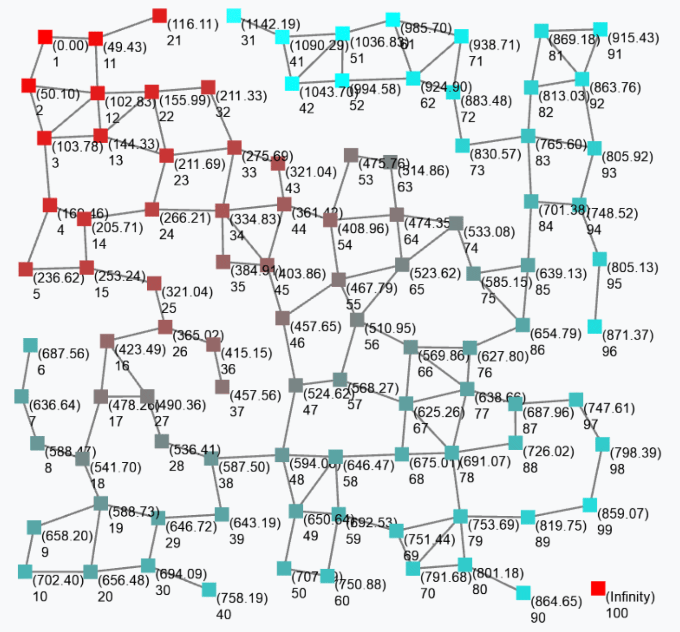
\includegraphics[width=\textwidth]{figures/gradient-example.png}
    \caption
    {
        A graphical representation of a gradient after stabilization.
        %
        Each device of the network is labelled with its distance from the source (in parenthesis) and its ID.
        %
        The source device is the one with ID 1.
        %
        Note that devices that are not connected to the source are considered to be at an infinite distance from it.
    }
    \label{fig:gradient}
\end{figure}
%
The implementation of a gradient using ScaFi is presented below.
%
\begin{lstlisting}[frame=single, language=scala]
def gradient(src: Boolean): Double =
  rep(Double.PositiveInfinity) { distance =>
    mux(src) {
      0.0
    } {
      minHoodPlus(nbr(distance) + nbrRange)
    }
  }
\end{lstlisting}
%
Some notes about the implementation:
%
\begin{itemize}
    \item \texttt{src} is an input field of source devices;
    \item the \texttt{mux} operator acts like an if statement where both branches get evaluated and end up in the export (unlike the \texttt{branch} construct, that only evaluates the side selected by the condition); this means that both source and non-source nodes will be aligned regardless of the chosen branch;
    \item \texttt{minHoodPlus} is an operator implemented in terms of \texttt{foldhood}, finding the minimum value for the given expression among neighbors;
    \item the \texttt{Plus} suffix of \texttt{minHood} indicates that the device itself is not considered during the calculation of the minimum, which for the gradient has the effect of preventing devices from getting stuck on low values after a source gets deactivated;
    \item \texttt{nbrRange} is a built-in neighboring sensor (implemented in terms of \texttt{nbrvar}) returning the estimated distance to the neighbor against which it is evaluated;
    \item source devices are at distance 0 from themselves, therefore the \quotes{then} branch of \texttt{mux} returns \texttt{0.0};
    \item at each device the gradient is calculated by repeatedly minimizing, for every neighbor, the sum of its currently estimated distance from the source (\texttt{nbr(distance)}) and the distance between the device and the neighbor (\texttt{nbrRange}).
\end{itemize}

\section{Proposed model}
\label{sec:proposed-model}

As stated before, in order to overcome the limitations of the proactive model this thesis proposes an approach based on \textit{reactivity}, leveraging the power of FRP (\Cref{sec:frp}) to deal with the complexity of the approach.
%
The sections below illustrate the objectives that are expected to be fulfilled by the final implementation and a high level description of the proposed reactive model.

\subsection{Objectives}
\label{sec:objectives}

The high level goal of this thesis is to provide a model that is expressive enough to allow developers to declaratively describe \textit{self-organizing} aggregate computations, while treating the dynamics and timing of relevant events as first class citizens.
%
This vision can be in fact summarized with \textit{functional reactive self-organization}.

The main objectives to be pursued in order to accomplish the goal are:
%
\begin{itemize}
    \item \textbf{Compute only upon relevant changes}: computations should occur reactively only when something changes in the environment, in order to avoid wasteful resources usage;
    \item \textbf{Broadcast messages only upon relevant changes}: each device should avoid broadcasting an export that did not change since the last one;
    \item \textbf{Avoid re-evaluation of unaffected sub-computations}: if a portion of the computation depends on data that did not change, it should not be re-evaluated.
\end{itemize}

\subsection{Reactive model}

The main difference between the model proposed by this thesis and the one proposed by field calculus is the \textit{absence of computation rounds}.
%
This is dictated by the fact that one of the objectives is to have computation run only upon relevant changes in the environment, namely:
%
\begin{itemize}
    \item a new device enters the neighborhood;
    \item a device leaves the neighborhood;
    \item an export coming from a neighbor is received;
    \item the value of a sensor changes;
    \item the value of a neighboring sensor changes.
\end{itemize}
%
Previously, these sources of events were all handled in the \textit{sense} stage of a computation round, and were all collected together in order to construct the \textit{context} for the round itself.
%
However, this was not done in a reactive fashion, since all these events were queued up while the device was sleeping and handled all at once at the start of the sense phase.
%
This meant that, if no event was received between two rounds, the computation would still happen.
%
The reactive model, instead, handles events as soon as they are received by the device (and only in that occasion), and only broadcasts the corresponding export if it is different than the previous, effectively fulfilling the \quotes{compute only upon relevant changes} and \quotes{broadcast messages only upon changes} objectives.

For what concerns the last objective (i.e., avoiding re-evaluating unaffected sub-computations), the optimized propagation of changes will be delegated to the correct use of the FRP engine and discussed further in \Cref{sec:specification}.

\section{Specification}
\label{sec:specification}

This section analyzes the key elements of the prototypal design for the reactive model.
%
Note that at this stage, the discussion is not tied to any particular technology, framework o programming language and should therefore be considered a \textit{specification} rather than a mirror of the actual code.
%
A deeper view on how this specification was translated into code can be found in \Cref{chap:implementation}.
% 
There is, however, a reference to Scala's data structures (e.g., \texttt{Map}s, \texttt{Option}s) and syntax for generics, which should not be considered as an enforcement on the usage of the Scala language.

\Cref{fig:class-diagram} shows a holistic picture of the proposed design, formalized as a UML class diagram.
%
The diagram does not show definitions for the types named \texttt{DeviceId}, \texttt{LocalSensorId} and \texttt{NeighborSensorId}.
%
This is a deliberate choice, since the specification does not depend on what those types really are.
%
Their only constraint is that it must be possible to tell if any two values of those types are equal with each other.
%
\begin{figure}
    \centering
    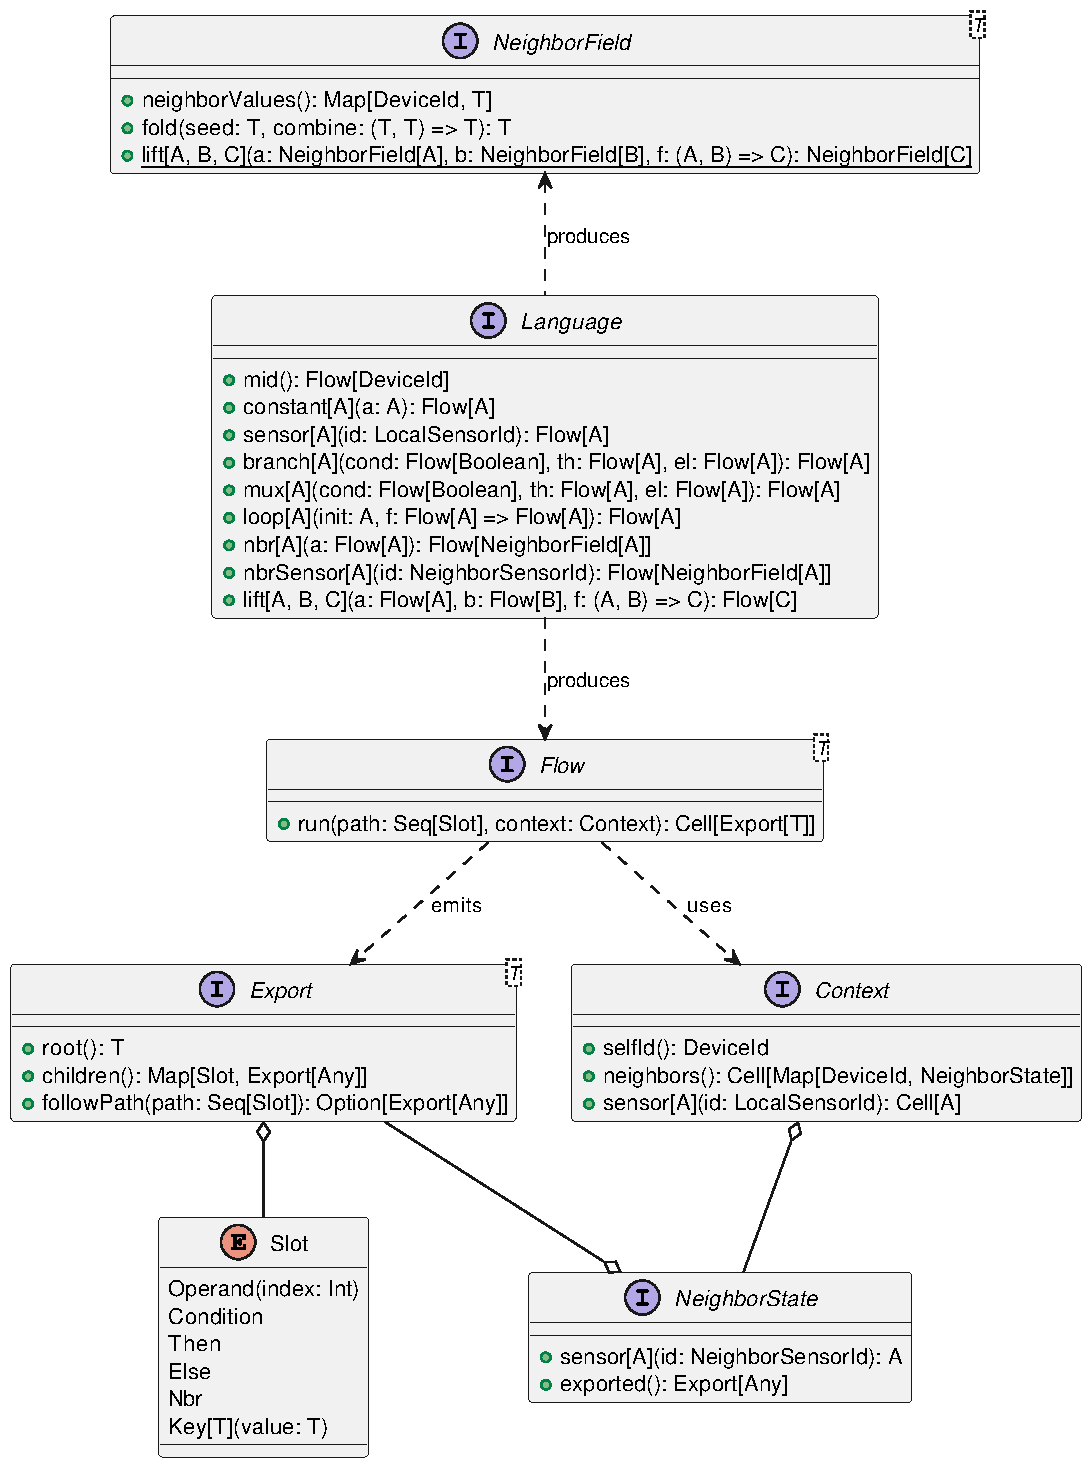
\includegraphics[width=0.95\textwidth]{figures/diagrams/specification.pdf}
    \caption{A class diagram of the specification of the reactive model.}
    \label{fig:class-diagram}
\end{figure}

The core of the specification starts from the definition of the \texttt{Context}, which is a way to express the environment where a device is immersed, and to provide handles for environmental changes to the computation.
%
In fact, this is done by expressing values that are subject to changes throughout the lifecycle of the system as cells.
%
In particular, sources of changes are:
%
\begin{itemize}
    \item local sensors
    \item neighbor devices information, which is expressed as a time-varying map from device identifiers to the last registered \texttt{NeighborState}, namely:
    \begin{itemize}
        \item the value for each neighboring sensor;
        \item the last export that was received.
    \end{itemize}
\end{itemize}
%
On top of that, the context is tied to the device identifier with which it is associated.

The \texttt{Export} that can be emitted by each device is represented as a tree where each child of a node is associated to a \texttt{Slot} that is unique among its siblings.
%
Being modeled this way, each sub-tree of the export is identified by a \textit{path} (i.e., a sequence of \texttt{Slot}s) starting from the root (an \textit{empty path}) and traversing the tree down to the node where it is rooted.
%
An example of this is shown in \Cref{fig:export-example}, which depicts the export of the following expression:
%
\begin{lstlisting}[frame=single]
branch(
  sensor[Boolean](SomeSensor),
  mux(
    sensor[Boolean](AnotherSensor),
    constant(1),
    constant(2)
  ),
  constant(0)
)
\end{lstlisting}
%
in a situation where \texttt{SomeSensor} evaluates to true and \texttt{AnotherSensor} evaluates to false.
%
Note that, for now, the semantics that lead to this particular shape of export are not relevant, as they will be discussed in detail in \Cref{sec:constructs-semantics}.
%
It is sufficient to know that each syntactic element of the expression above (with the exception of \texttt{constant(0)} which is excluded due to branching) corresponds to some path inside the tree, as follows:
%
\begin{verbatim}
[]                  <=>  branch(...)
[Condition]         <=>  sensor[Boolean](SomeSensor)
[Then]              <=>  mux(...)
[Then / Condition]  <=>  sensor[Boolean](AnotherSensor)
[Then / Then]       <=>  constant(1)
[Then / Else]       <=>  constant(2)
\end{verbatim}
%
\begin{figure}
    \centering
    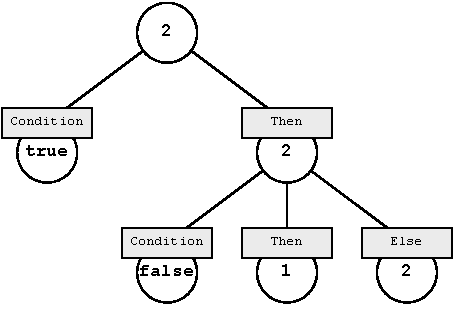
\includegraphics[width=0.6\textwidth]{figures/export-example.pdf}
    \caption{An example of an export. Circles represent nodes, while rectangles represent slots.}
    \label{fig:export-example}
\end{figure}
%
This representation of an export is essential to perform the \textit{alignment} process.
%
In fact, two exports are aligned at a certain path if and only if that path exists in both exports.

All the constructs of the \texttt{Language} deal with \texttt{Flow}s, a type which is designed to encapsulate aggregate (sub-)computations as a dependency graph (in a way that's closely related to the dependency graph of an FRP engine).
%
A \texttt{Flow}, in fact, is essentially a function that takes a path and a \texttt{Context} and returns a cell of \texttt{Export}s, possibly depending on the exports of other \texttt{Flow}s recursively.
%
The path represents the point in the evaluation tree where that \texttt{Flow} is placed, while the \texttt{Context} places the computation inside some device.
%
Notice that this design of a \texttt{Flow} has some consequences:
%
\begin{itemize}
    \item since the context is passed to it after its construction and the output is a cell, a \texttt{Flow} effectively represents an entire aggregate computation, independent of space and time;
    \item since exports are returned as a cell, all (sub-)computations are automatically updated when the original sources of events are updated by the context;
    \item due to the fact that the path is also passed when requesting the cell of exports, the same instance of a \texttt{Flow} can be used multiple times in different points of the same computation, making it referentially transparent;
    \item since FRP is used under the hood, the requirement of functions passed to operators of the language being referentially transparent still exists;
    \item the main expression of an aggregate program should be evaluated from the empty path.
\end{itemize}

An important difference from the model used by ScaFi is the presence of a \textit{reified} \texttt{NeighborField} type, that is used as the returned type of operators that deal with the neighborhood, i.e., \texttt{nbr} and \texttt{nbrSensor}.
%
A \texttt{NeighborField} is essentially a wrapper around a map from neighbor identifiers to local values, which can be folded over in order to collapse all local values into a single one.

\subsection{Constructs semantics}
\label{sec:constructs-semantics}

This section presents the semantics of the constructs belonging to the \texttt{Language} interface.
%
Here, the term semantics is used to refer to the way the flow generated by each construct produces its exports from its inputs, depicted in a visual fashion.
%
Note that these rules are to be interpreted as snapshots, and thus they should be re-applied on each new evaluation of the corresponding cell.

Some graphical notations are:
%
\begin{itemize}
    \item expressions may use variables to capture arguments that are passed;
    \item a variable typed as a \texttt{Flow} may be used in a graph as the current export for that flow at the path where it is rooted;
    \item sub-exports may be represented as triangles when their content is not relevant;
    \item \texttt{r(\_)} expresses the value contained in the root of an export;
    \item \texttt{N(\_)} expresses the collection of all the given expressions for each aligned neighbor (graphically shown with arrows);
    \item \texttt{E(\_)} denotes an atomic export whose root is the given argument;
    \item \texttt{ctx.xyz} corresponds to member \texttt{xyz} of the \texttt{Context} on which the flow is run;
    \item \texttt{nbr.xyz} refers to member \texttt{xyz} of the current neighbor being evaluated inside of \texttt{N(\_)}.
\end{itemize}

The simplest constructs of the language are those that are local and atomic (i.e., they work without knowledge of neighbors and they do not depend on other flows).
%
These are described in \Cref{fig:semantics-local-atomic}.
%
Being atomic, their corresponding trees only contain a root node with the final value of the expression:
\begin{itemize}
    \item \texttt{constant} defines a constant flow and always evaluates to the argument that has been passed;
    \item \texttt{mid} is a constant flow of device identifiers always evaluates to the \texttt{selfId} returned by the \texttt{Context};
    \item \texttt{sensor} implements the sensing abilities of each device uses the cell returned by the \texttt{Context} for the given sensor identifier;
\end{itemize}
%
\begin{figure}
    \centering
    \begin{subfigure}[b]{0.3\textwidth}
        \centering
        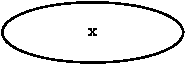
\includegraphics[width=\textwidth]{figures/semantics/constant.pdf}
        \caption{\texttt{constant(x)}}
        \label{fig:semantics-constant}
    \end{subfigure}
    \hfill
    \begin{subfigure}[b]{0.3\textwidth}
        \centering
        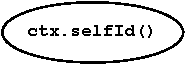
\includegraphics[width=\textwidth]{figures/semantics/mid.pdf}
        \caption{\texttt{mid()}}
        \label{fig:semantics-mid}
    \end{subfigure}
    \hfill
    \begin{subfigure}[b]{0.3\textwidth}
        \centering
        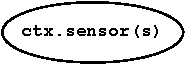
\includegraphics[width=\textwidth]{figures/semantics/sensor.pdf}
        \caption{\texttt{sensor(s)}}
        \label{fig:semantics-sensor}
    \end{subfigure}
    \caption{Semantics of the atomic constructs.}
    \label{fig:semantics-local-atomic}
\end{figure}

The \texttt{branch} construct (\Cref{fig:semantics-branch}) corresponds to the \textit{if} construct of field calculus and works in such a way that, for a given expression \texttt{branch(c, t, e)}, only the export selected by \texttt{c} is included in the final output.
%
In cases where the condition is true, \texttt{t} is included under the \texttt{Then} slot and its root is used as the global root, otherwise \texttt{e} is included under the \texttt{Else} slot and its root is used instead.
%
In both cases, \texttt{c} is inserted under the \texttt{Condition} slot.
%
With this semantics, any sub-computation under \texttt{t} or \texttt{e} will not align with any neighbor executing the opposite branch, due to the fact that their paths will differ at the \texttt{Then}/\texttt{Else} slot.
%
\begin{figure}
    \centering
    \begin{subfigure}[b]{0.40\textwidth}
        \centering
        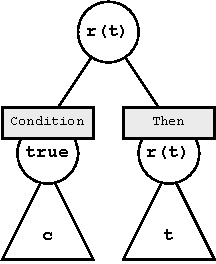
\includegraphics[width=\textwidth]{figures/semantics/branch-true.pdf}
        \caption{\texttt{true} condition.}
        \label{fig:semantics-branch-true}
    \end{subfigure}
    \hfill
    \begin{subfigure}[b]{0.40\textwidth}
        \centering
        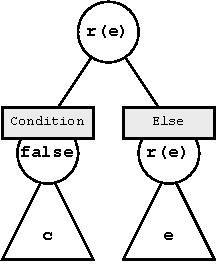
\includegraphics[width=\textwidth]{figures/semantics/branch-false.pdf}
        \caption{\texttt{false} condition.}
        \label{fig:semantics-branch-false}
    \end{subfigure}
    \caption{Semantics of \texttt{branch(c, t, e)}.}
    \label{fig:semantics-branch}
\end{figure}

The \texttt{mux} operator (\Cref{fig:semantics-mux}) is an alternative to \texttt{branch} that introduces conditional behavior without resulting in partitions in the device network.
%
That is, devices running sub-computations in \texttt{t} or \texttt{e} will always align with each other since both exports will be included in the final one, respectively under the \texttt{Then} and \texttt{Else} slots.
%
\begin{figure}
    \centering
    \begin{subfigure}[b]{0.47\textwidth}
        \centering
        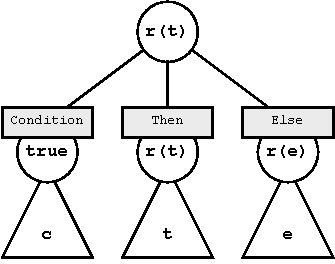
\includegraphics[width=\textwidth]{figures/semantics/mux-true.pdf}
        \caption{\texttt{true} condition.}
        \label{fig:semantics-mux-true}
    \end{subfigure}
    \hfill
    \begin{subfigure}[b]{0.47\textwidth}
        \centering
        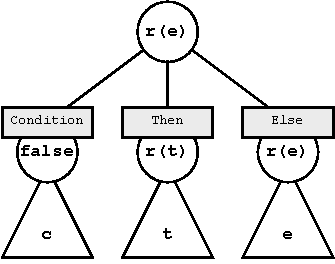
\includegraphics[width=\textwidth]{figures/semantics/mux-false.pdf}
        \caption{\texttt{false} condition.}
        \label{fig:semantics-mux-false}
    \end{subfigure}
    \caption{Semantics of \texttt{mux(c, t, e)}.}
    \label{fig:semantics-mux}
\end{figure}

Neighboring constructs, i.e., \texttt{nbr} and \texttt{nbrSensor}, require knowing which neighbors are aligned when they get evaluated, as shown in \Cref{fig:semantics-neighboring}.
%
This means that, if this constructs are used at a certain path \texttt{p}, the engine should filter out all neighbors whose known export does not contain \texttt{p}.
%
Furthermore, only the sub-exports rooted at \texttt{p} of each neighbor need to be considered.
%
The \texttt{nbr(a)} constructs works by collecting all neighboring values of \texttt{a}, which can be found at \texttt{p / Nbr} for each neighbor.
%
Since every device is a neighbor of itself, this process should also take care of replacing the value produced by the previous evaluation with the new value coming from \texttt{a}.
%
This is shown in \Cref{fig:semantics-nbr} by the isolated arrow going from \texttt{r(a)} in the current device to the root of the export.
%
For what concerns \texttt{nbrSensor}, the engine just uses the current \texttt{NeighborState} of each aligned neighbor to evaluate the sensor with the specified identifier.
%
\begin{figure}
    \centering
    \begin{subfigure}[b]{0.47\textwidth}
        \centering
        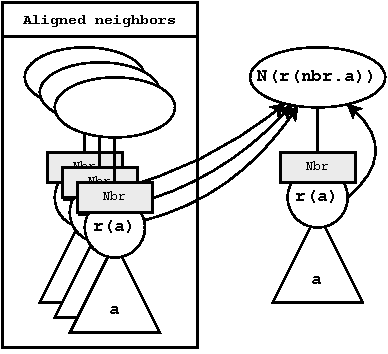
\includegraphics[width=\textwidth]{figures/semantics/nbr.pdf}
        \caption{\texttt{nbr(a)}}
        \label{fig:semantics-nbr}
    \end{subfigure}
    \hfill
    \begin{subfigure}[b]{0.47\textwidth}
        \centering
        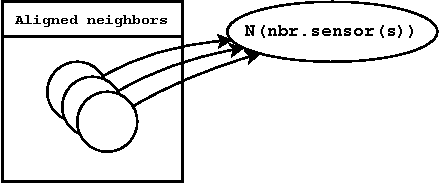
\includegraphics[width=\textwidth]{figures/semantics/nbrSensor.pdf}
        \caption{\texttt{nbrSensor(s)}}
        \label{fig:semantics-nbrsensor}
    \end{subfigure}
    \caption{Semantics of neighboring constructs.}
    \label{fig:semantics-neighboring}
\end{figure}

The language also defines a \texttt{lift} construct.
%
\textit{Lifting} is a well-known concept of functional programming that allows a function working with atomic values to be applied to wrapped versions of those values, for some wrapper type.
%
In this case, the wrapper type is the \texttt{Flow} type, and lifting a function to the \texttt{Flow} world means producing another \texttt{Flow} obtained by applying that function to the roots of those flows, and having the original exports as children of the resulting one.
%
This is shown in \Cref{fig:semantics-lift}, which depicts the case where \texttt{f} is a binary function (the generalization to n-ary functions is in fact trivial).
%
\begin{figure}
    \centering
    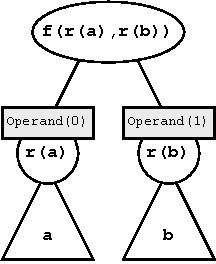
\includegraphics[width=0.4\textwidth]{figures/semantics/lift.pdf}
    \caption{Semantics of \texttt{lift(a, b, f)}.}
    \label{fig:semantics-lift}
\end{figure}

As a side note, the specification also defines a \texttt{lift} operation on instances of \texttt{NeighborField}s.
%
It has the effect of evaluating the given function on pairs of values associated with the same device and returning the outputs as another \texttt{NeighborField}.

The final construct is \texttt{loop}.
%
This is designed to be an adaptation of \texttt{rep} as defined by field calculus to the reactive model.
%
This change was necessary due to the fact that \texttt{rep} is based on the underlying execution model structured in computation rounds, but that's not the case in the reactive model.
%
Instead of using proactive and repeated application of a function, \texttt{loop} manages field evolution over time as a reaction to changes in the previous state.
%
Other than the initial state, \texttt{loop} accepts a function transforming a \texttt{Flow} into another \texttt{Flow} of the same type.
%
These \texttt{Flow}s shall be interpreted as the input always being \quotes{one step behind} the output.
%
The specification states that the \quotes{off-by-one} \texttt{Flow} should be constructed by aligning with the previous state of the same device, which can be read from the context leveraging the fact that the every device is a neighbor of itself (\Cref{fig:semantics-loop-next}).
%
In cases where alignment is not possible (i.e., on the first evaluation or after a switch of branch), the first argument of loop should be used to construct a new export (\Cref{fig:semantics-loop-init}).
%
The implementation should take care of the following caveats arising from the intrinsic self-dependency of \texttt{loop}:
%
\begin{itemize}
    \item \textit{infinite recursion}: since computations are triggered by themselves changing in the past, \texttt{loop} should not cause \textit{stack overflows} and therefore should use some sort of \textit{rate-limiting} strategy (e.g., \textit{throttling});
    \item \textit{indefinite export growth}: a flow defined in terms of itself might cause the export tree to grow on each update, since exports are are repeatedly wrapped in other exports; the implementation should take care of passing an \textit{atomic} flow as an input to the subsequent computation, in order to avoid indefinite growth.
\end{itemize}
%
\begin{figure}
    \centering
    \begin{subfigure}[b]{0.47\textwidth}
        \centering
        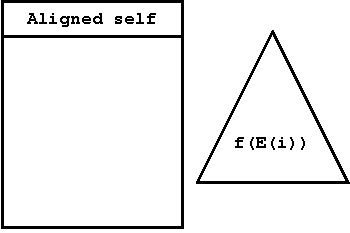
\includegraphics[width=\textwidth]{figures/semantics/loop-init.pdf}
        \caption{Not aligned with previous state}
        \label{fig:semantics-loop-init}
    \end{subfigure}
    \hfill
    \begin{subfigure}[b]{0.47\textwidth}
        \centering
        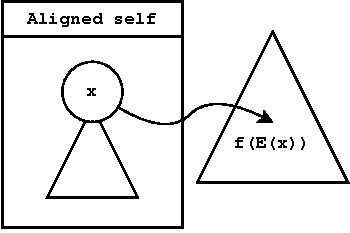
\includegraphics[width=\textwidth]{figures/semantics/loop-next.pdf}
        \caption{Aligned with previous state}
        \label{fig:semantics-loop-next}
    \end{subfigure}
    \caption{Semantics of \texttt{loop(i, f)}.}
    \label{fig:semantics-loop}
\end{figure}
